% =============================================================================
%  CHƯƠNG 3 – PHƯƠNG PHÁP ĐỀ XUẤT MADDPG
% =============================================================================
\chapter{PHƯƠNG PHÁP ĐỀ XUẤT MADDPG}
\label{ch:chuong3}

Chương này trình bày chi tiết phương pháp đề xuất của Luận văn để giải
bài toán surrogate của P0 \eqref{eq:P0}: Khuôn khổ MADDPG ba tác tử
chuyên dụng với cơ chế CTDE, kèm theo ba cải tiến chính: (i) tham số
hóa pha residual dựa trên nghiệm phân tích bậc một; (ii) hàm phần
thưởng Lagrangian surrogate với các biến đối ngẫu $\lambda_k$ per-user
cập nhật bằng projected dual gradient; và (iii) lịch trình heuristic
hai pha (two-stage dual freeze) giúp phần thưởng trở nên dừng
(stationary) ở giai đoạn cuối huấn luyện, nhờ đó đường cong huấn luyện
dễ diễn giải.

% -----------------------------------------------------------------------------
\section{Tổng quan kiến trúc MADDPG-CTDE đề xuất}
\label{sec:maddpg_overview}

\subsection{Sơ đồ tổng thể}

Như đã trình bày ở mục \ref{sec:maddpg} của Chương 1, MADDPG sử dụng cơ
chế huấn luyện tập trung, thực thi phân tán (CTDE)
\cite{lowe2017multi}. Trong giai đoạn huấn luyện, mỗi tác tử có một
Actor cục bộ và chia sẻ một Critic tập trung, vì vậy Critic luôn quan
sát đầy đủ trạng thái và hành động của toàn hệ thống, đảm bảo môi trường
ổn định từ góc nhìn của Critic. Trong giai đoạn thực thi, Critic được bỏ
đi; mỗi Actor chỉ cần quan sát cục bộ để sinh hành động.

Khuôn khổ MADDPG đề xuất trong Luận văn được thiết kế đặc thù cho bài
toán P0 với ba tác tử chuyên dụng:
\begin{itemize}[leftmargin=*]
\item \textbf{Tác tử 0, BS Power Agent:} điều khiển phân bổ công suất
$\{P_c, P_1, \ldots, P_K\}$ và tỷ lệ tách $\{c_1, \ldots, c_K\}$.
\item \textbf{Tác tử 1, STAR-RIS Reflection Agent:} điều khiển pha
$\{\theta_n^R\}$ và biên độ $\{\beta_n^R\}$ phản xạ.
\item \textbf{Tác tử 2, STAR-RIS Transmission Agent:} điều khiển pha
$\{\theta_n^T\}$ truyền qua (biên độ $\beta_n^T = 1 - \beta_n^R$ được
suy ra từ ràng buộc bảo toàn năng lượng).
\end{itemize}

\subsection{Lý do phân rã thành ba tác tử chuyên dụng}

So với cách triển khai một tác tử duy nhất với không gian hành động hợp
nhất 140 chiều, hoặc cách triển khai $N$ tác tử (mỗi phần tử RIS một tác
tử), khuôn khổ ba tác tử chuyên dụng có ba ưu điểm
\cite{lowe2017multi}, \cite{dange2026collaborative}, \cite{mirza2024multi}:

\textbf{(i) Mỗi tác tử có vai trò chức năng rõ ràng,} dễ phân tích và gỡ
lỗi. Tác tử BS chỉ tập trung vào tài nguyên thời gian-công suất, các tác
tử STAR-RIS chỉ tập trung vào tài nguyên không gian (pha-biên độ).

\textbf{(ii) Không gian hành động của mỗi tác tử nhỏ vừa phải,} dễ huấn
luyện hơn so với một tác tử 140 chiều. Đồng thời, số tác tử vừa đủ
(3) để Critic tập trung không gặp vấn đề chiều cao.

\textbf{(iii) Tách biệt được thông tin quan sát.} Tác tử BS không cần
biết chi tiết kênh BS-RIS-UE; tác tử RIS-R không cần biết tốc độ tổng
hiện tại. Điều này giảm chiều quan sát của từng tác tử, đẩy nhanh học.

% -----------------------------------------------------------------------------
\section{Kiến trúc mạng nơ-ron}
\label{sec:nn_architecture}

\subsection{Mạng Actor}

Mỗi tác tử $i \in \{0, 1, 2\}$ có một mạng Actor
$\mu_i: \R^{|o_i|} \to \R^{|a_i|}$ với kiến trúc multi-layer
perceptron (MLP) ba lớp \cite{lillicrap2016continuous}:
\begin{equation}
\mu_i(o_i) = \tanh\!\big(W^{(3)}_i\,\sigma(\mathrm{LN}(W^{(2)}_i\,
            \sigma(\mathrm{LN}(W^{(1)}_i\,o_i + b^{(1)}_i)) + b^{(2)}_i))
            + b^{(3)}_i\big),
\label{eq:actor_nn}
\end{equation}
trong đó $\sigma(\cdot) = \mathrm{ReLU}(\cdot)$ là hàm kích hoạt phi
tuyến, $\mathrm{LN}(\cdot)$ là chuẩn hóa lớp (LayerNorm) giúp ổn định
huấn luyện, và $\tanh$ ở lớp cuối ép đầu ra vào $[-1, 1]$.

Kích thước các lớp ẩn được đặt cố định ở $256$ đơn vị cho mọi Actor, một
giá trị đã được nghiên cứu chứng minh là cân bằng giữa năng lực biểu
diễn và chi phí tính toán \cite{lillicrap2016continuous}, \cite{fujimoto2018addressing}.
Cụ thể:
\begin{itemize}[leftmargin=*]
\item Actor 0 (BS): $26 \to 256 \to 256 \to 9$
\item Actor 1 (RIS-R): $344 \to 256 \to 256 \to 64$
\item Actor 2 (RIS-T): $180 \to 256 \to 256 \to 32$
\end{itemize}

Các trọng số được khởi tạo theo phương pháp orthogonal với gain
$1{,}0$ cho các lớp ẩn và gain $0{,}01$ cho lớp đầu ra, một thủ thuật
giúp tránh saturation tanh ở giai đoạn đầu huấn luyện.

\subsection{Mạng Critic tập trung}

Mỗi tác tử $i \in \{0, 1, 2\}$ có một mạng Critic riêng
$Q_i: \R^{681} \times \R^{140} \to \R$ nhận vào toàn bộ quan sát ghép
$(o_0, o_1, o_2)$ và toàn bộ hành động ghép $(a_0, a_1, a_2)$:
\begin{equation}
Q_i(\mathbf{o}, \mathbf{a}; \phi_i) =
W^{(3)}_i\,\sigma(\mathrm{LN}(W^{(2)}_i\,
\sigma(\mathrm{LN}(W^{(1)}_i\,[\mathbf{o}; \mathbf{a}] + b^{(1)}_i)) + b^{(2)}_i))
+ b^{(3)}_i.
\label{eq:critic_nn}
\end{equation}
Kích thước mỗi Critic: $821 \to 256 \to 256 \to 1$, không có activation
cuối (Q-value là giá trị thực không bị giới hạn).

\textbf{Tại sao dùng ba Critic riêng dù phần thưởng chung?} Trong khuôn
khổ cooperative MARL với phần thưởng $r_t$ chia sẻ cho tất cả tác tử
(mục \ref{sec:adaptive_reward}), về mặt lý thuyết một Critic chung là đủ
vì các tác tử có cùng giá trị mục tiêu. Tuy nhiên Luận văn vẫn duy trì
ba Critic riêng theo công thức MADDPG gốc \cite{lowe2017multi}
vì hai lý do thực tiễn:
\begin{itemize}[leftmargin=*]
\item Linh hoạt cho mở rộng: ba Critic riêng cho phép dễ dàng
chuyển sang kịch bản phần thưởng không đồng nhất trong tương lai
(ví dụ: tác tử BS quan tâm sum-rate, tác tử RIS-R quan tâm fairness cục
bộ vùng R, v.v.) mà không cần thay đổi kiến trúc.
\item Giảm phương sai gradient: dù phần thưởng chung, mỗi Critic
hội tụ về cùng giá trị $Q^*$ theo các quỹ đạo ngẫu nhiên khác nhau
(khởi tạo, batch sampling). Trung bình của ba gradient Critic cho Actor
tương ứng được quan sát ổn định hơn so với một Critic chung trong các
thí nghiệm sơ bộ.
\end{itemize}
\textbf{Chi phí:} ba Critic làm tăng số tham số tổng thể khoảng $3\times$
so với một Critic chung, nhưng do Critic chỉ dùng trong giai đoạn huấn
luyện (không cần khi triển khai), chi phí này không ảnh hưởng đến độ
trễ suy luận.

\subsection{Mạng mục tiêu (Target networks)}

Để ổn định mục tiêu Bellman trong huấn luyện, mỗi mạng Actor và Critic
đều có một bản sao mạng mục tiêu $\mu_i'$, $Q_i'$ được cập nhật
mềm sau mỗi bước:
\begin{equation}
\theta_i' \leftarrow \tau\,\theta_i + (1 - \tau)\,\theta_i', \quad
\phi_i' \leftarrow \tau\,\phi_i + (1 - \tau)\,\phi_i',
\label{eq:soft_update}
\end{equation}
với $\tau = 0{,}005$ là hệ số cập nhật mềm rất nhỏ. Cập nhật này đảm bảo
mạng mục tiêu thay đổi chậm hơn rất nhiều so với mạng học, tạo môi
trường ``ổn định ngắn hạn'' để Critic hội tụ.

% -----------------------------------------------------------------------------
\section{Ánh xạ pha STAR-RIS và ablation residual}
\label{sec:residual_phase}

Trong cấu hình chính đã đăng ký trước, đầu ra Actor pha $a_n^X\in[-1,1]$
được ánh xạ tuyệt đối theo
\begin{equation}
  \theta_n^X = \pi(a_n^X+1) \pmod{2\pi}, \qquad X\in\{R,T\}.
\end{equation}
Cách ánh xạ này không phụ thuộc baseline giải tích và là cấu hình duy nhất
được dùng cho ma trận kết quả chính. Một biến thể residual có thể được khảo
sát riêng:
\begin{equation}
  \theta_n^X = \big[\theta_{n,\mathrm{prior}}^X
  + \rho_{\phi}\pi a_n^X\big]_{2\pi}.
\end{equation}
Prior phải được tính nhất quán từ phương trình tín hiệu thu MISO. Biến thể
residual là một ablation tùy chọn; mọi lựa chọn $\rho_{\phi}$ phải được khóa
bằng validation trước khi mở test bank và không được trình bày như đóng góp
thực nghiệm của cấu hình absolute.

\section{Hàm phần thưởng Lagrangian surrogate và cập nhật đối ngẫu per-user}
\label{sec:adaptive_reward}

\subsection{Vấn đề khi dùng phần thưởng đơn giản}

Phần thưởng đơn giản $r_t = R_{\text{sum}}$ \cite{hieu2021optimal} có hai
nhược điểm trong bài toán P0:

\textbf{(i) Không khuyến khích thỏa mãn QoS.} Vì tổng $R_{\text{sum}}$ có
thể đạt cao mà vẫn có UE chịu tốc độ thấp hơn $R_{\min}$, tác tử có xu
hướng bỏ qua UE yếu để tối đa tổng tốc độ, vi phạm ràng buộc (C4).

\textbf{(ii) Cân bằng cứng giữa sum-rate và QoS.} Một phần thưởng dạng
$r = R_{\text{sum}} - \lambda \cdot \text{penalty}$ với $\lambda$ cố
định sẽ phụ thuộc vào việc chọn $\lambda$ tốt: $\lambda$ quá nhỏ thì
penalty bị bỏ qua, $\lambda$ quá lớn thì tác tử bỏ qua sum-rate.

\subsection{Công thức Lagrangian surrogate}

Luận văn dùng hàm phần thưởng \eqref{eq:reward} đã phát biểu ở Chương 2,
với thang đo và giới hạn:
\begin{equation}
r_t \;=\; \mathrm{clip}\!\Big(0{,}1 \cdot \big(r^{\text{sr}}_t + r^{\text{dual}}_t
                                    + r^{\text{aug}}_t + r^{\text{sw}}_t\big),\,
                              -50,\, +50\Big),
\label{eq:reward_full}
\end{equation}
với bốn thành phần:

\textbf{(1) Thành phần sum-rate chuẩn hóa:}
\begin{equation}
r^{\text{sr}}_t = \alpha\,\frac{R_{\text{sum},t}}{R_{\text{ref}}},\quad
\alpha = 1{,}5,\; R_{\text{ref}} = 20 \text{ b/s/Hz}.
\label{eq:r_sr}
\end{equation}

\textbf{(2) Thành phần đối ngẫu bậc nhất (dấu đầy đủ):} với hàm ràng buộc
$c_{k,t} = R_{\min} - R_{k,t}$,
\begin{equation}
r^{\text{dual}}_t = -\sum_{k=1}^{K} \lambda_k\, c_{k,t}.
\label{eq:r_dual}
\end{equation}
Số hạng này dùng $c_k$ \emph{có dấu} như trong Lagrangian chuẩn: khi
người dùng $k$ dư QoS ($c_k < 0$), tích $\lambda_k c_k$ âm và thành phần
đóng góp dương, đúng bản chất bù trừ của biến đối ngẫu.

\textbf{(3) Thành phần phạt bậc hai tăng cường (augmented):}
\begin{equation}
r^{\text{aug}}_t = -\frac{w}{2}\sum_{k=1}^{K}\!\big[\max(0,\,c_{k,t})\big]^2,
\quad w = 1{,}0,
\label{eq:r_aug}
\end{equation}
chỉ tác dụng lên phần vi phạm, làm trơn vùng lân cận biên ràng buộc.

\textbf{(4) Thành phần chi phí tái cấu hình (switching cost):}
\begin{equation}
r^{\text{sw}}_t = -\eta_{\phi}\,\overline{\big(1-\cos\Delta\phi_n\big)}
                  -\eta_{P}\,\frac{\lVert\Delta\mathbf{w}^{P}\rVert_1}{K+1}
                  -\eta_{\beta}\,\overline{\lvert\Delta\beta_n\rvert},
\label{eq:r_switch}
\end{equation}
trong đó $\Delta$ so với hành động vật lý đã áp ở bước trước (bằng $0$
tại $t=0$); dấu gạch ngang là trung bình theo số phần tử. Chi phí này
phản ánh giá phải trả khi tái cấu hình STAR-RIS/công suất giữa hai khối
coherence, đồng thời làm cho hành động hiện tại ảnh hưởng thực sự tới
các bước sau (tính chất MDP).

Hai lưu ý so với các thiết kế trước: (i) số hạng phạt vượt công suất bị
loại bỏ vì phép tham số hóa softmax bảo đảm
$P_c + \sum_k P_k = P_{\max}$ theo cấu trúc, khiến số hạng này luôn
bằng không (số hạng ``chết''); (ii) thành phần thưởng nhị phân theo tỷ
lệ UE đạt QoS chỉ còn là tùy chọn ablation
(\texttt{enable\_qos\_shaping\_bonus}, mặc định tắt) vì nó làm méo
gradient quanh biên ràng buộc.

\subsection{Cập nhật đối ngẫu có phép chiếu (projected dual gradient)}
\label{sec:dual_update}

Mỗi người dùng có một biến đối ngẫu riêng $\lambda_k \geq 0$. Cuối mỗi
episode, gọi $\bar{c}_k$ là trung bình episode của $c_{k,t}$ và
$\hat{c}_k$ là trung bình trượt mũ (EMA) của $\bar{c}_k$ với hệ số
$0{,}9$; cập nhật:
\begin{equation}
\lambda_k \;\leftarrow\; \Pi_{[0,\,\lambda_{\max}]}
\big[\lambda_k + \eta_{\lambda}\, \hat{c}_k\big],
\qquad \eta_{\lambda} = 0{,}01,\; \lambda_{\max} = 20,
\label{eq:lambda_update}
\end{equation}
với $\Pi$ là phép chiếu lên đoạn $[0, \lambda_{\max}]$. Vì $\hat{c}_k$
có dấu, $\lambda_k$ tăng khi người dùng $k$ vi phạm kỳ vọng
($\hat{c}_k > 0$) và \emph{giảm} khi có slack ($\hat{c}_k < 0$) --- đây
là gradient ascent trên hàm đối ngẫu của bài toán ràng buộc kỳ vọng
$\max \mathbb{E}[R_{\text{sum}}]$ s.t. $\mathbb{E}[c_k] \leq 0$, thực
hiện riêng cho từng ràng buộc.

\subsection{Lịch trình hai pha đóng băng biến đối ngẫu (two-stage dual freeze)}
\label{sec:freeze_lambda}

Cập nhật \eqref{eq:lambda_update} có một hệ quả phụ quan
trọng: vì $\lambda_k$ thay đổi theo thời gian, \emph{thang đo của hàm
phần thưởng} \eqref{eq:reward_full} cũng thay đổi theo, khiến mục tiêu
học của tác tử trở nên không dừng (non-stationary). Hệ quả là đường
cong tổng phần thưởng (Return) khó đạt trạng thái phẳng ngay cả khi
chính sách đã ổn định.

Để xử lý, Luận văn dùng một \emph{lịch trình heuristic hai pha}
(two-stage dual freeze):
\begin{equation}
\boldsymbol{\lambda}_{t+1} =
\begin{cases}
\text{cập nhật theo \eqref{eq:lambda_update}}, & t < \rho_f \cdot E \\
\boldsymbol{\lambda}_t \ (\text{đóng băng}),   & t \geq \rho_f \cdot E
\end{cases}
\label{eq:lambda_freeze}
\end{equation}
với $E$ là tổng số episode và $\rho_f = 0{,}55$. Trong pha một,
$\lambda_k$ được điều chỉnh bằng gradient đối ngẫu; trong pha hai,
$\lambda_k$ giữ cố định để hàm phần thưởng dừng và đường cong Return dễ
diễn giải. Cần nhấn mạnh hai điểm trung thực về mặt phương pháp:
(i) việc đóng băng là một \emph{heuristic ổn định hóa}, không phải một
cơ chế có bảo đảm hội tụ; toàn bộ quy trình
\eqref{eq:lambda_update}--\eqref{eq:lambda_freeze} \emph{không} được
tuyên bố hội tụ về điểm yên ngựa của Lagrangian; và (ii) vùng phẳng của
đường cong Return trong pha hai chỉ cho thấy phần thưởng đã dừng,
\emph{không tự nó chứng minh} chính sách đã hội tụ về nghiệm tối ưu.
Mốc đóng băng được đặt sau thời điểm nhiễu khám phá OU về sàn (mục
\ref{sec:training}). Cơ chế này áp dụng thống nhất cho cả các thuật
toán DRL để bảo đảm so sánh công bằng.

\subsection{Phần thưởng chia sẻ}

Trong khuôn khổ cooperative MARL, cả ba tác tử nhận cùng một
phần thưởng $r_t$. Điều này khuyến khích các tác tử phối hợp với nhau:
tác tử BS phân bổ công suất sao cho khả thi với pha mà tác tử RIS-R và
RIS-T chọn, và ngược lại.

\subsection{Vì sao phạt cố định không tối ưu}
\label{sec:why_fixed_fails}

Một câu hỏi thiết yếu về thiết kế là: tại sao không sử dụng hệ số phạt
$\lambda$ cố định? Phân tích lý thuyết và thực nghiệm dưới đây làm rõ
nguyên nhân.

Với $\lambda$ cố định, phần thưởng trở thành tổng có trọng số cứng giữa
sum-rate và phạt vi phạm QoS. Khi phân phối kênh thay đổi giữa các
episode, mức độ khó của ràng buộc QoS cũng thay đổi: trong các channel
realization có $|h_{\text{eff},k}|$ lớn, ràng buộc QoS dễ thỏa và phạt
cao gây áp lực dư thừa làm suy giảm sum-rate; ngược lại, trong các
realization khó, phạt thấp khiến tác tử bỏ qua QoS để khai thác
sum-rate. Đây là biểu hiện điển hình của vấn đề
\emph{reward shaping tĩnh}: một hệ số trọng số không thể đồng thời tối
ưu trên một phân phối đa dạng.

Về mặt lý thuyết, hàm phần thưởng
\eqref{eq:reward_full} là Lagrangian (tăng cường) của bài toán tối ưu
có ràng buộc kỳ vọng:
\begin{equation}
\max\;\E[R_{\text{sum}}] \quad \text{s.t.}\quad
\E[c_k] \leq 0,\;\; k = 1, \ldots, K,
\label{eq:constrained_problem}
\end{equation}
tức mỗi người dùng có một ràng buộc kỳ vọng riêng. Bộ nhân tử tối ưu
$\lambda_k^\star$ phụ thuộc vào phân phối kênh và mức độ bó chặt của
từng ràng buộc, không phải là hằng số chung. Việc chọn $\lambda$ cố
định (và chung cho mọi người dùng) tương đương giả định trước bộ nhân
tử, dẫn đến điểm dừng suboptimal.

\subsection{Trực giác cân bằng throughput-QoS}
\label{sec:tradeoff_intuition}

Cập nhật \eqref{eq:lambda_update} chính là gradient ascent có phép
chiếu trên hàm đối ngẫu của \eqref{eq:constrained_problem}: gradient
của hàm đối ngẫu theo $\lambda_k$ là $\E[c_k]$, được ước lượng bằng
trung bình episode (làm trơn EMA), và phép chiếu giữ
$\lambda_k \in [0, \lambda_{\max}]$. Trực giác: khi ràng buộc của người
dùng $k$ bị vi phạm theo kỳ vọng, $\lambda_k$ tăng làm chính sách
chuyển ưu tiên sang người dùng đó; khi có slack, $\lambda_k$ giảm để
giải phóng dung lượng cho sum-rate. Tuy nhiên, vì bài toán primal
(chính sách mạng nơ-ron, mục tiêu phi lồi) không được giải tới tối ưu
giữa hai lần cập nhật đối ngẫu, quy trình tổng thể là một phép xấp xỉ
thực dụng: Luận văn \emph{không} tuyên bố hội tụ điểm yên ngựa hay
khoảng cách đối ngẫu (duality gap) bằng không; hành vi của
$\boldsymbol{\lambda}$ được báo cáo bằng thực nghiệm (Hình
\ref{fig:qos_lambda}) với từng $\lambda_k$ được ghi log riêng.

% -----------------------------------------------------------------------------
\section{Cập nhật mạng và Quy trình huấn luyện}
\label{sec:training}

\subsection{Hàm mất mát Critic và cập nhật Actor}

Tại mỗi bước cập nhật, MADDPG lấy một mini-batch
$\mathcal{B} = \{(\mathbf{o}, \mathbf{a}, r, \mathbf{o}')\}$ kích thước $256$
từ replay buffer $\mathcal{D}$ (kích thước $300\,000$ chuyển tiếp). Mục
tiêu Bellman cho Critic là:
\begin{equation}
y_i = r + \gamma\,Q_i'\!\big(\mathbf{o}',\, \mu_0'(o_0'),\, \mu_1'(o_1'),\,
                              \mu_2'(o_2');\,\phi_i'\big),
\label{eq:bellman_target}
\end{equation}
với $\gamma = 0{,}95$ là hệ số chiết khấu. Hàm mất mát Critic:
\begin{equation}
\mathcal{L}_{\text{critic}}(\phi_i) =
\frac{1}{|\mathcal{B}|}\sum_{\mathcal{B}}
\big(Q_i(\mathbf{o}, \mathbf{a}; \phi_i) - y_i\big)^2.
\label{eq:critic_loss}
\end{equation}
Hàm mục tiêu cho Actor $\mu_i$ (DPG):
\begin{equation}
\nabla_{\theta_i} J(\mu_i) =
\E_{\mathcal{B}}\!\left[\nabla_{a_i} Q_i(\mathbf{o}, a_0, \ldots, a_{N-1}; \phi_i)
                         \big|_{a_i = \mu_i(o_i)}\,
                         \nabla_{\theta_i} \mu_i(o_i)\right].
\label{eq:actor_gradient}
\end{equation}
Optimizer Adam được sử dụng với learning rate $10^{-4}$ cho Actor và
$5 \times 10^{-4}$ cho Critic. Gradient được clip bởi norm $1{,}0$
để tránh nổ gradient.

\subsection{Khám phá: nhiễu Ornstein--Uhlenbeck}

Để khuyến khích khám phá hành động liên tục, một quá trình
Ornstein--Uhlenbeck (OU) được thêm vào đầu ra Actor trong giai đoạn
huấn luyện \cite{lillicrap2016continuous}:
\begin{equation}
\tilde a_t = \mu_i(o_i) + \mathcal{N}_t^{\text{OU}}, \quad
\mathcal{N}_t^{\text{OU}} = \mathcal{N}_{t-1}^{\text{OU}} + \theta_{\text{OU}}(0 - \mathcal{N}_{t-1}^{\text{OU}}) + \sigma_t\,\xi_t,
\end{equation}
với $\xi_t \sim \mathcal{N}(0, I)$. Tham số $\sigma_t$ giảm tuyến tính từ
$\sigma_0 = 0{,}4$ về $\sigma_f = 0{,}05$ trong $45\,000$ bước đầu tiên
(tương ứng episode $\approx 900$), sau đó giữ cố định. Sự suy giảm này
thực hiện cân bằng exploration--exploitation: ban đầu khám phá rộng,
sau khi đã có chính sách tương đối tốt thì khai thác. Mốc nhiễu về sàn
được đặt \emph{trước} mốc đóng băng $\lambda$ (episode $1\,100$, mục
\ref{sec:freeze_lambda}) để giai đoạn cuối huấn luyện đồng thời là pha
khai thác thuần túy trên hàm phần thưởng dừng.

\subsection{Warmup ngẫu nhiên}

Trong $5\,000$ bước đầu tiên, tác tử lấy hành động ngẫu nhiên đồng
đều thay vì dùng Actor. Mục đích là làm đầy replay buffer với các mẫu
đa dạng trước khi bắt đầu cập nhật mạng, tránh việc Actor bị thiên kiến
ngay từ đầu do dữ liệu nghèo nàn.

\subsection{Sơ đồ luồng thuật toán huấn luyện}
\label{sec:algo_workflow}

Trước khi trình bày dạng pseudo-code chính thức, Hình
\ref{fig:algo_workflow} mô tả trực quan luồng huấn luyện MADDPG đề
xuất dưới dạng flowchart. Sơ đồ này giúp nắm bắt cấu trúc tổng thể
trước khi đi vào chi tiết kỹ thuật.

\begin{figure}[H]
  \centering
  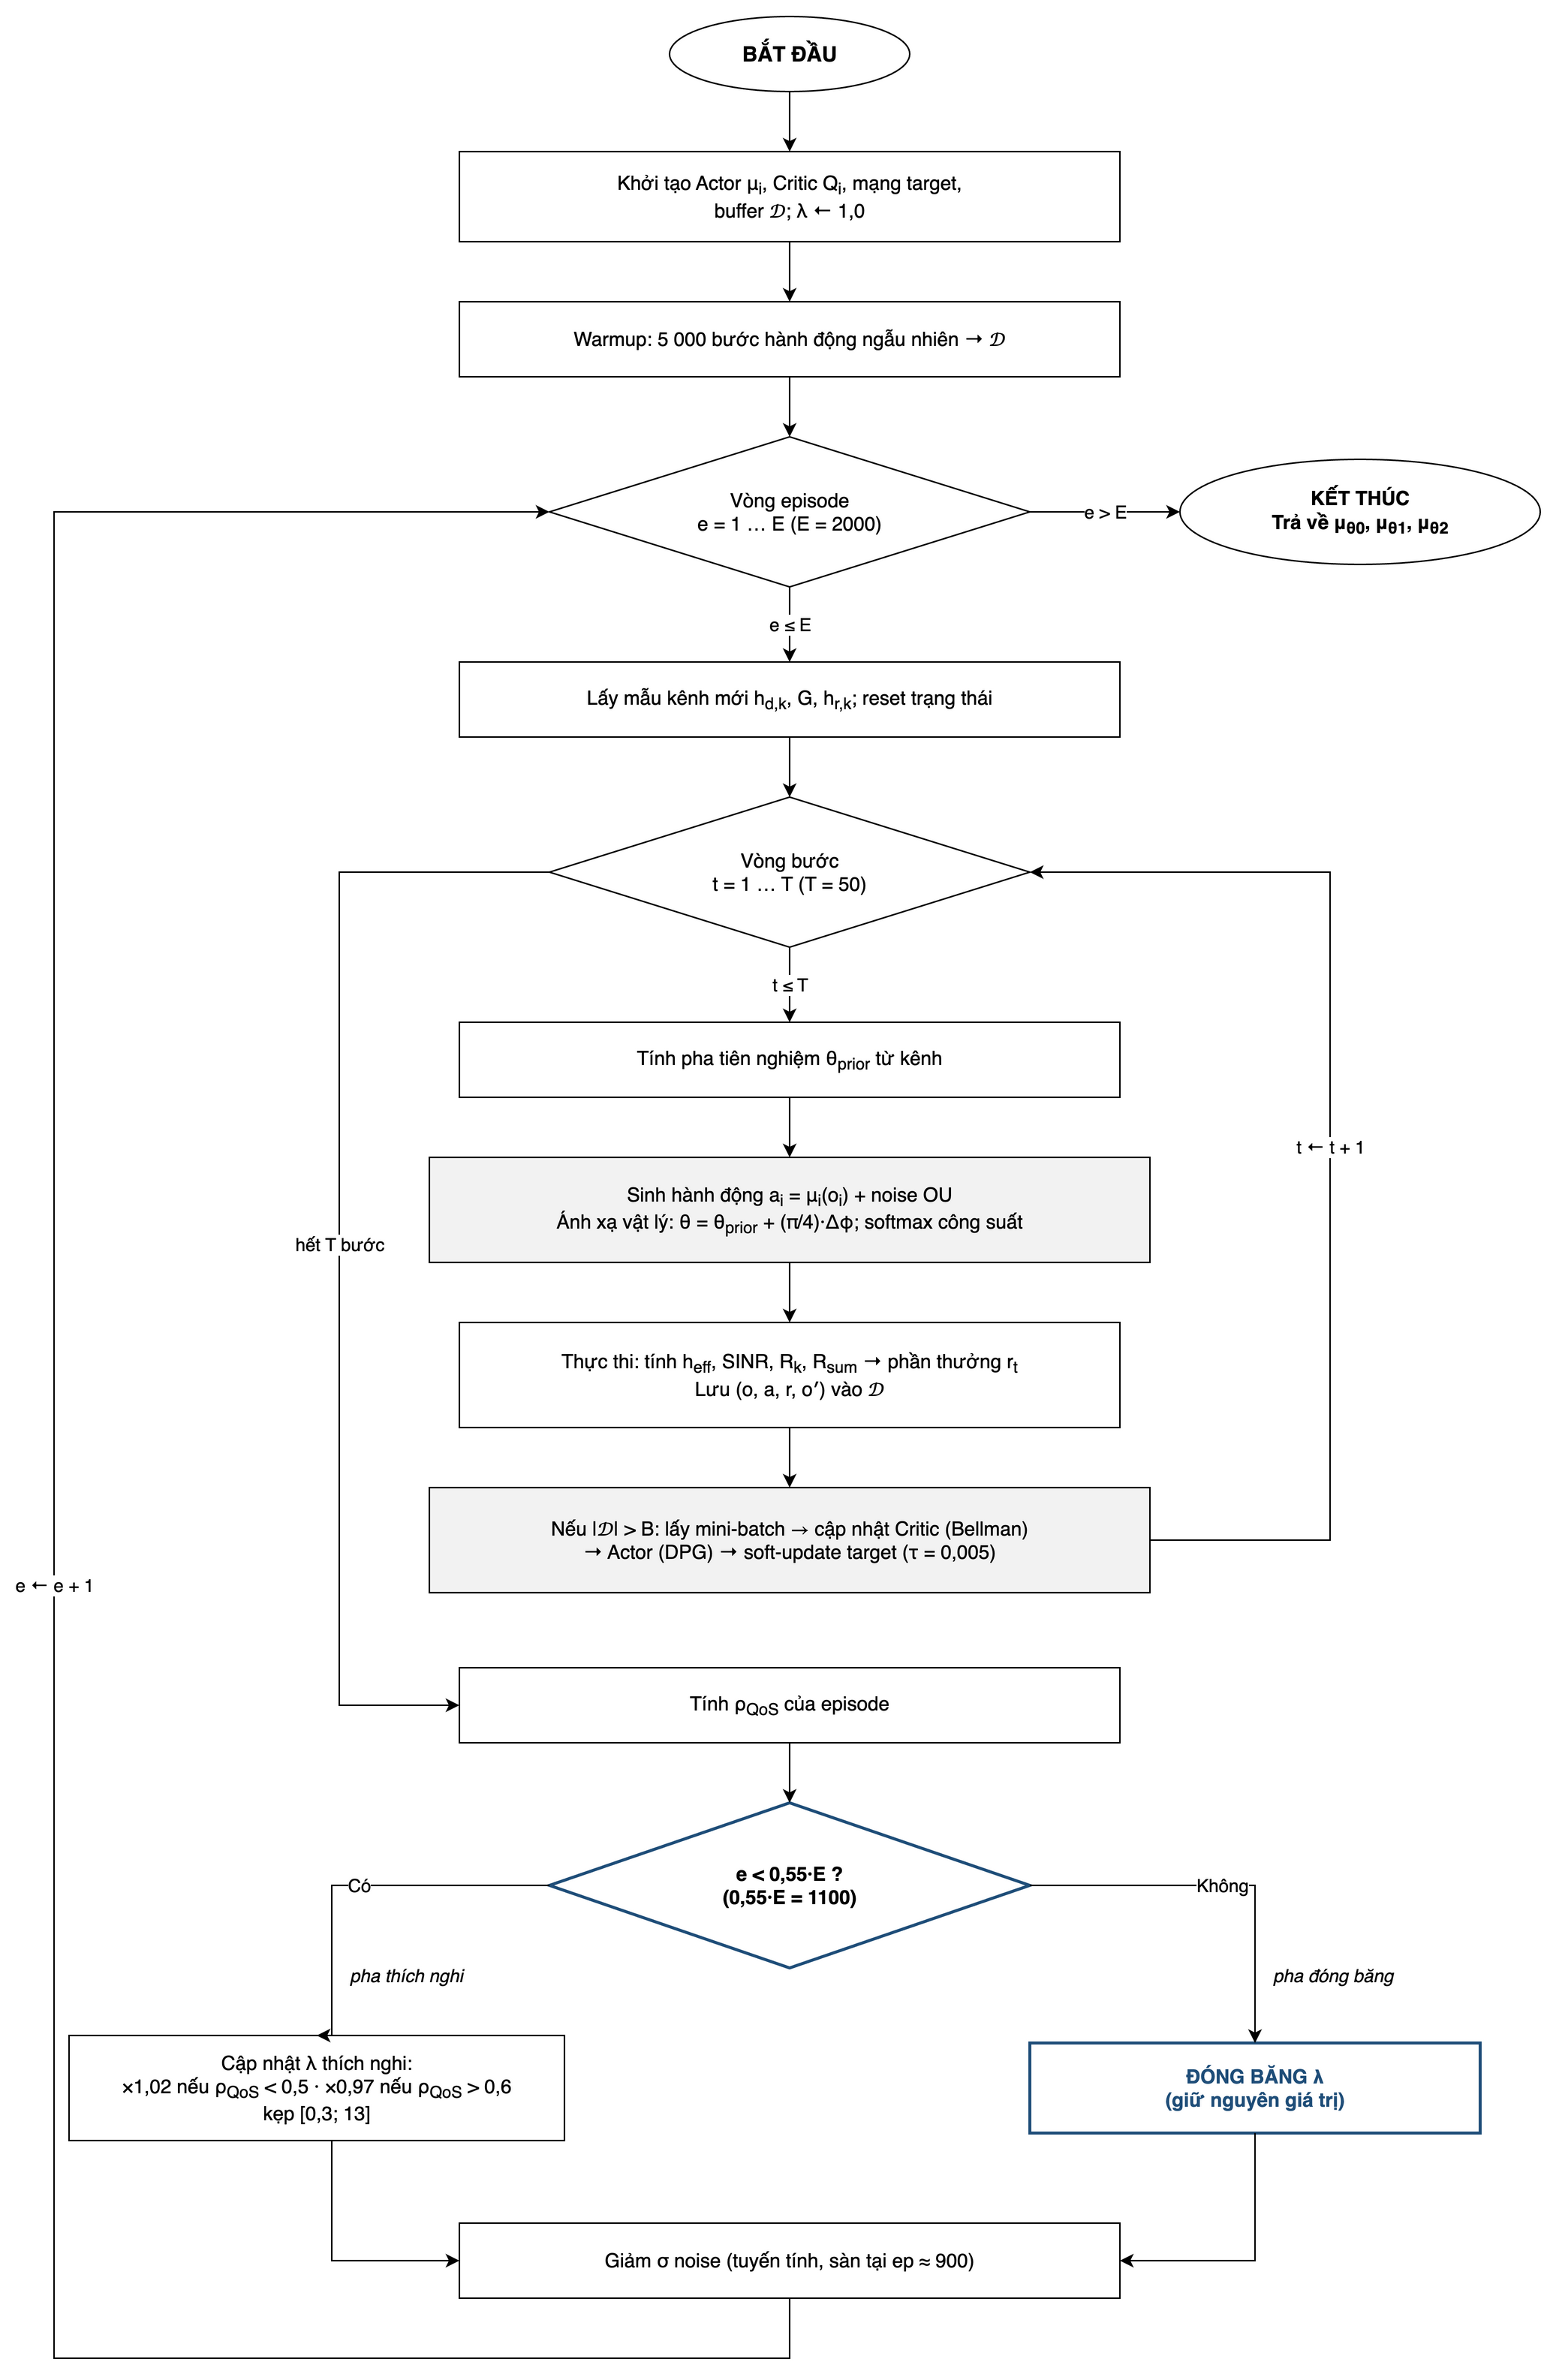
\includegraphics[width=0.78\linewidth]{figures/h3_algorithm_flowchart.png}
  \caption{Sơ đồ luồng thuật toán huấn luyện MADDPG đề xuất, gồm 13
  bước chính từ khởi tạo, warmup, vòng episode lồng vòng step, đến
  cập nhật mạng và hệ số phạt Lagrangian $\lambda$.}
  \label{fig:algo_workflow}
\end{figure}

Sơ đồ phân tách rõ hai vòng lặp lồng nhau: vòng ngoài duyệt qua $E$
episode (mỗi episode: hình học người dùng mới và trạng thái kênh khởi
tạo mới), vòng trong duyệt $T$ khối coherence; trong mỗi khối, tác tử
quan sát kênh hiện hành, ra một quyết định, nhận phần thưởng trên kênh
đó, rồi kênh tiến hóa Gauss--Markov sang khối kế tiếp
\eqref{eq:gauss_markov}. Các khối tô màu đậm (các bước 8 và 12) đánh
dấu các bước có liên quan đến mạng nơ-ron: sinh hành động và cập nhật
Actor-Critic. Các khối còn lại tương ứng với các phép tính kênh truyền,
phần thưởng và quản lý bộ đệm phát lại. Cập nhật các biến đối ngẫu
$\lambda_k$ (bước 13) diễn ra ở cuối mỗi episode theo
\eqref{eq:lambda_update}.

\subsection{Thuật toán huấn luyện chính thức (Algorithm 1)}

\begin{algorithm}[H]
\caption{Proposed MADDPG-Based STAR-RIS RSMA Optimization}
\label{alg:maddpg_train}
\begin{algorithmic}[1]
\Require Số episode $E$, độ dài episode $T$, batch size $B$, kích thước
buffer $|\mathcal{D}|_{\max}$, learning rate $\eta_a, \eta_c$, hệ số
chiết khấu $\gamma$, hệ số cập nhật mềm $\tau$, hệ số phạt khởi tạo
$\lambda_0$, OU noise $\sigma_0 \to \sigma_f$, số bước warmup $T_w$
\Ensure Các Actor đã huấn luyện $\mu_{\theta_0}, \mu_{\theta_1}, \mu_{\theta_2}$
\Statex \textit{// Khởi tạo}
\State Khởi tạo trọng số $\theta_i$ cho Actor $\mu_i$ và $\phi_i$ cho Critic $Q_i$, $i \in \{0, 1, 2\}$
\State Khởi tạo mạng mục tiêu: $\theta_i' \leftarrow \theta_i$, $\phi_i' \leftarrow \phi_i$
\State Khởi tạo replay buffer $\mathcal{D} \leftarrow \emptyset$, $\lambda \leftarrow \lambda_0$
\Statex \textit{// Giai đoạn warmup}
\State Thu thập $T_w = 5{,}000$ chuyển tiếp với hành động ngẫu nhiên đồng đều, lưu vào $\mathcal{D}$
\Statex \textit{// Vòng lặp huấn luyện chính}
\For{$\text{episode} = 1, 2, \ldots, E$}
  \State Lấy mẫu hình học người dùng mới; khởi tạo kênh $h_{d,k}, \mathbf{G}, \mathbf{h}_{r,k}^X \sim \mathcal{CN}(\cdot)$
  \State Khởi tạo trạng thái: $o_{i,1}$ cho $i \in \{0, 1, 2\}$
  \For{$t = 1, 2, \ldots, T$}\Comment{mỗi $t$ là một khối coherence}
    \State Tính tiên nghiệm pha $\theta_n^{\text{prior},X}$ theo công thức \eqref{eq:phase_prior}
    \State $a_{i,t} \leftarrow \mu_{\theta_i}(o_{i,t}) + \mathcal{N}_t^{\text{OU}}$, $i \in \{0, 1, 2\}$
    \State Map $a_{i,t}$ thành tham số vật lý: $\{P_c, P_k, c_k\}$, $\{\theta_n^X, \beta_n^R\}$
    \State Thực thi $\mathbf{a}_t$ trên kênh hiện hành, tính $h_{\text{eff},k}$, $R_k$, $R_{\text{sum}}$
    \State Tính phần thưởng $r_t$ theo \eqref{eq:reward_full} (gồm chi phí tái cấu hình so với $\mathbf{a}_{t-1}$)
    \State Tiến hóa kênh sang khối kế tiếp theo \eqref{eq:gauss_markov}
    \State Lưu chuyển tiếp $(\mathbf{o}_t, \mathbf{a}_t, r_t, \mathbf{o}_{t+1})$ (quan sát THÔ) vào $\mathcal{D}$
    \If{$|\mathcal{D}| > B$}
      \State Lấy mini-batch $\mathcal{B} = \{(\mathbf{o}, \mathbf{a}, r, \mathbf{o}')\}_{j=1}^B$ từ $\mathcal{D}$
      \For{$i \in \{0, 1, 2\}$}
        \State Tính mục tiêu Bellman: $y_i \leftarrow r + \gamma\, Q_{\phi_i'}\!\big(\mathbf{o}', \mu_{\theta_0'}(o_0'), \ldots\big)$
        \State Cập nhật Critic: $\phi_i \leftarrow \phi_i - \eta_c \nabla_{\phi_i} \mathcal{L}_i$ theo \eqref{eq:critic_loss}
        \State Cập nhật Actor: $\theta_i \leftarrow \theta_i + \eta_a \nabla_{\theta_i} J$ theo \eqref{eq:actor_gradient}
        \State Cập nhật mạng mục tiêu: $\theta_i' \leftarrow \tau \theta_i + (1-\tau)\theta_i'$; $\phi_i'$ tương tự
      \EndFor
    \EndIf
  \EndFor
  \State Tính trung bình episode của khe hở ràng buộc: $\bar{c}_k = \frac{1}{T}\sum_t (R_{\min} - R_{k,t})$
  \State Cập nhật $\lambda_k$ theo lịch hai pha \eqref{eq:lambda_freeze}: projected dual gradient \eqref{eq:lambda_update} nếu $\text{episode} < \rho_f E$, ngược lại đóng băng
  \State Giảm OU noise: $\sigma_t$ theo lịch tuyến tính từ $\sigma_0$ về $\sigma_f$
\EndFor
\State \Return $\mu_{\theta_0}, \mu_{\theta_1}, \mu_{\theta_2}$
\end{algorithmic}
\end{algorithm}

% -----------------------------------------------------------------------------
\section{Bảng siêu tham số tổng kết}
\label{sec:hyperparameters}

Bảng \ref{tab:hyperparameters} liệt kê toàn bộ siêu tham số sử dụng để
huấn luyện MADDPG, được chia thành các nhóm: tham số học (learning rate,
hệ số chiết khấu, kích thước batch), tham số khám phá (nhiễu OU, số bước
decay), tham số mạng nơ-ron (kích thước lớp ẩn, activation, gradient
clip) và tham số phần thưởng Lagrangian thích nghi. Các giá trị này
được lựa chọn dựa trên kinh nghiệm thực nghiệm và các khuyến nghị trong
tài liệu chuẩn về DDPG/MADDPG.

\begin{table}[t]
\centering
\caption{Siêu tham số huấn luyện MADDPG-CTDE đề xuất.}
\label{tab:hyperparameters}
\begin{tabular}{p{5.5cm} l}
\toprule
\textbf{Siêu tham số} & \textbf{Giá trị} \\
\midrule
Số episode huấn luyện               & $E = 2\,000$ \\
Độ dài mỗi episode                  & $T = 50$ khối coherence \\
Hệ số tương quan kênh Gauss--Markov & $\rho = 0{,}95$ \\
Số hạt giống huấn luyện             & $8$ \\
Số bước warmup ngẫu nhiên           & $5\,000$ \\
Mốc đóng băng normalizer quan sát   & $5\,000$ bước môi trường \\
Tổng số chuyển tiếp huấn luyện      & $100\,000$ / hạt giống \\
Kích thước replay buffer            & $|\mathcal{D}| = 300\,000$ (quan sát thô) \\
Batch size                          & $B = 256$ \\
Hệ số chiết khấu                    & $\gamma = 0{,}95$ \\
Hệ số cập nhật mềm                  & $\tau = 0{,}005$ \\
Learning rate Actor                 & $\eta_a = 10^{-4}$ \\
Learning rate Critic                & $\eta_c = 5 \times 10^{-4}$ \\
Số lớp ẩn                           & $2$ (mỗi lớp $256$ đơn vị) \\
Activation                          & ReLU + LayerNorm \\
Output activation Actor             & tanh \\
Gradient clip (norm)                & $1{,}0$ \\
Nhiễu OU $\sigma_0 \to \sigma_f$    & $0{,}4 \to 0{,}05$ \\
Số bước decay nhiễu                 & $45\,000$ (episode $\approx 900$) \\
Ánh xạ pha cấu hình chính          & Pha tuyệt đối, $	heta_n=\pi(a_n+1)$ \\
$\lambda_k$ ban đầu                 & $1{,}0$ (mỗi người dùng) \\
Miền chiếu $\lambda_k$              & $[0,\, 20]$ \\
Tốc độ học đối ngẫu $\eta_{\lambda}$ & $0{,}01$ (EMA $0{,}9$) \\
Tỷ lệ đóng băng $\lambda$ ($\rho_f$) & $0{,}55$ (episode $1\,100$) \\
Hệ số $\alpha$ sum-rate / $R_{\text{ref}}$ & $1{,}5$ / $20$ b/s/Hz \\
Trọng số augmented penalty $w$      & $1{,}0$ \\
Trọng số switching cost $\eta_{\phi}/\eta_{P}/\eta_{\beta}$ & $0{,}1 / 0{,}05 / 0{,}05$ \\
Reward clip                         & $[-50,\, +50]$ \\
\bottomrule
\end{tabular}
\end{table}

% -----------------------------------------------------------------------------
\section{Phân tích độ phức tạp tính toán}
\label{sec:complexity}

\subsection{Độ phức tạp huấn luyện}

Mỗi bước cập nhật yêu cầu một lần chạy tiến/ngược qua các Actor và Critic.
Với 3 tác tử và Critic kích thước $821 \to 256 \to 256 \to 1$:
\begin{equation}
\mathcal{C}_{\text{train,step}} = O\!\big(3 \times (256^2 + 256 \times 821)\big)
                                = O(10^5)\ \text{ops}.
\end{equation}
Tổng cộng $100\,000$ bước cập nhật mỗi hạt giống cho thấy chi phí huấn
luyện vào khoảng $10^{10}$ phép toán nổi, tương đương vài giờ trên CPU
thông thường hoặc dưới một giờ trên GPU phổ thông (đo thực tế ở pipeline
cũ: $\approx 40$ phút/hạt giống trên GPU T4).

\subsection{Độ phức tạp suy luận}

Tại thời điểm thực thi, chỉ Actor được dùng:
\begin{equation}
\mathcal{C}_{\text{infer}} = O\!\big(|o_i| \times 256 + 256^2 + 256 \times |a_i|\big)
                            \approx O(10^4)\ \text{ops/agent}.
\end{equation}
Mỗi khối coherence chỉ cần đúng một lần suy luận (một quyết định cho
một khối), nên độ trễ suy luận cỡ mili-giây là phù hợp với nhịp cập
nhật theo khối pha-đinh (vài ms tới hàng chục ms). Độ trễ được đo bằng
hai benchmark riêng biệt --- CPU (một luồng, ép toàn bộ mô hình về CPU)
và GPU (đồng bộ hóa CUDA quanh vùng đo) --- trình bày ở Chương 4; hai
bảng không được so sánh trực tiếp với nhau. Số đo tham chiếu của
pipeline cũ ($\approx 1{,}3$ ms/hành động) được thực hiện với
device=auto (GPU T4) nên chỉ có giá trị định hướng; kết luận chính
thức dùng cặp bảng CPU/GPU mới.

% -----------------------------------------------------------------------------
\section*{Kết luận chương}
\addcontentsline{toc}{section}{Kết luận chương}

Chương 3 đã trình bày chi tiết khuôn khổ MADDPG-CTDE ba tác tử chuyên
dụng để giải bài toán surrogate của P0. Ba cải tiến quan trọng được đề
xuất: (i) ánh xạ pha tuyệt đối nhất quán với cấu hình đã khóa
$4^N$ lần và cung cấp một điểm khởi đầu hợp lý; (ii) hàm phần thưởng
Lagrangian surrogate với các biến đối ngẫu $\lambda_k$ per-user cập
nhật bằng projected dual gradient trên khe hở ràng buộc có dấu, tự điều
chỉnh cân bằng giữa tổng tốc độ và mức đáp ứng QoS; (iii) lịch trình
heuristic hai pha đóng băng $\boldsymbol{\lambda}$ (two-stage dual
freeze) làm cho hàm phần thưởng trở nên dừng ở $45\%$ cuối huấn luyện,
giúp đường cong huấn luyện dễ diễn giải (không phải một bảo đảm hội
tụ). Cùng với các
kỹ thuật chuẩn (replay buffer, target networks, OU noise, warmup,
gradient clip), khuôn khổ đề xuất hội tụ ổn định và đạt hiệu năng
cạnh tranh, điều sẽ được kiểm chứng thực nghiệm ở Chương 4 --- bao gồm
cả thí nghiệm khả năng mở rộng theo số phần tử $N$ nhằm định lượng
lợi thế của kiến trúc phân rã đa tác tử.
